\documentclass{beamer}
\mode<presentation> {
\usetheme{Boadilla}
}

%%import packages....I didnt use all of these, they're just in my template
\usepackage{graphicx}
\usepackage{booktabs}
\usepackage{standalone}
\usepackage{tikz}
\usepackage{textpos}
\usepackage{modiagram}
\usepackage{physics}
\usepackage{amsmath}
\usepackage[percent]{overpic}
\usepackage{subfig}
\usepackage{xcolor}
\usepackage{subfiles}



\usetikzlibrary{arrows.meta,positioning,decorations.markings,backgrounds}

\tikzset{
    every node/.style={font=\footnotesize},
}

%%citation style parameters

\usepackage[backend=bibtex,%
isbn=false,%
url=false,%
style=authoryear,%
% firstinits=false,
maxbibnames=2,%
]{biblatex}
\bibliography{My Collection.bib}

\renewbibmacro*{cite}{%
  \iffieldundef{shorthand}
    {\ifthenelse{\ifnameundef{labelname}\OR\iffieldundef{labelyear}}
       {\usebibmacro{cite:label}%
        \setunit{\printdelim{nonameyeardelim}}}
       {\printnames{labelname}%
        \setunit{\printdelim{nameyeardelim}}}%
     \usebibmacro{cite:labeldate+extradate}%
     \setunit{\addcomma\space}%
     \usebibmacro{journal}}
    {\usebibmacro{cite:shorthand}}}



%I dont remember why I have this in my template
\usetikzlibrary{decorations.pathreplacing,angles,quotes}

%%UNT color scheme
\colorlet{beamer@blendedblue}{green!40!black}

% Title Information
\title[LIBS]{Sputtering Targets}
\author{Brian Squires}
\institute[UNT]
{
University of North Texas \\
\medskip
\textit{Department of Physics}\\
\medskip
\textit{brian.squires@unt.edu}\\
\medskip
\textit{}
}
\date{\today}
% \logo{\vspace{7.25cm}\includegraphics[height=1.5cm]{/Users/briansquires/github/logo1.jpg}}

%Add shaded outline slide before each section
\AtBeginSection[]
{
    \begin{frame}
        \frametitle{Outline}
        \tableofcontents[currentsection]
    \end{frame}
}


\begin{document}
\begin{frame}
    \titlepage    
\end{frame}

\begin{frame}{Average Linewidth = 0.9996nm}
    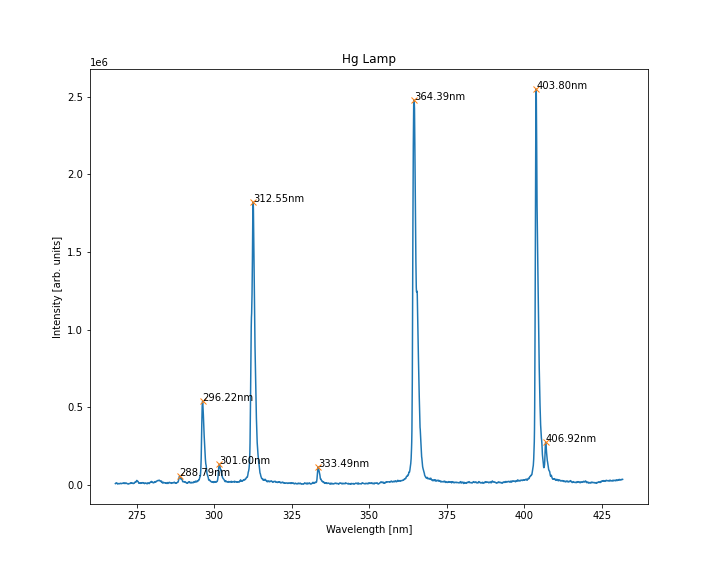
\includegraphics[scale=0.45]{calibrationlamp.png}
\end{frame}

\begin{frame}
    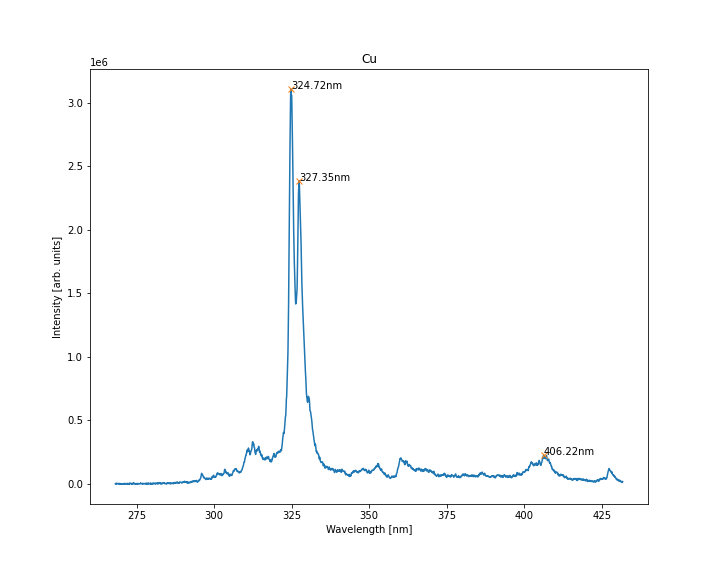
\includegraphics[scale=0.45]{Cu/Cu_350.png}
\end{frame}

\begin{frame}
    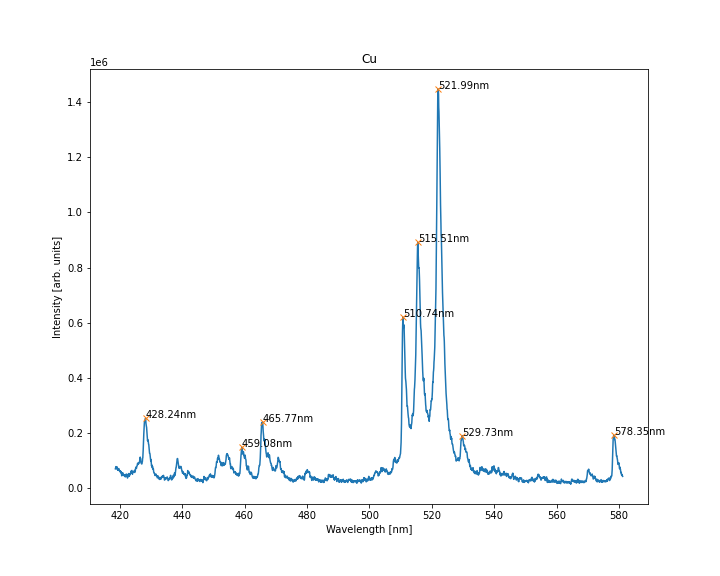
\includegraphics[scale=0.45]{Cu/Cu_500.png}
\end{frame}

\begin{frame}
    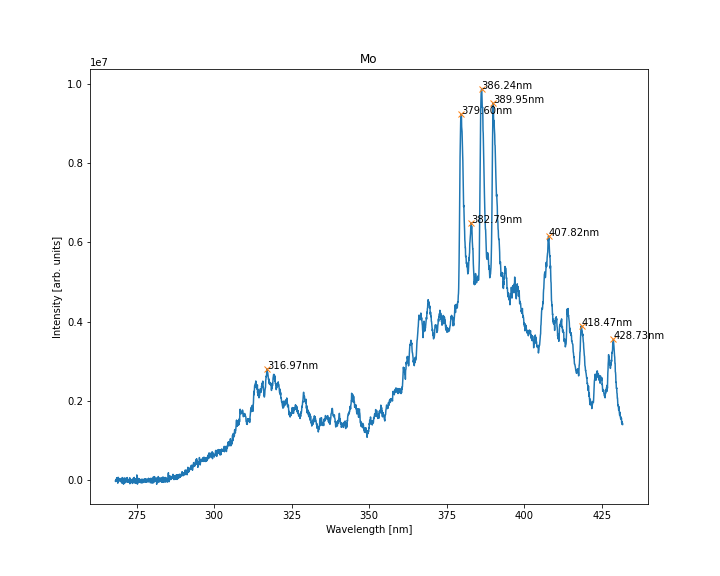
\includegraphics[scale=0.45]{Mo/Mo_350.png}
\end{frame}

\begin{frame}
    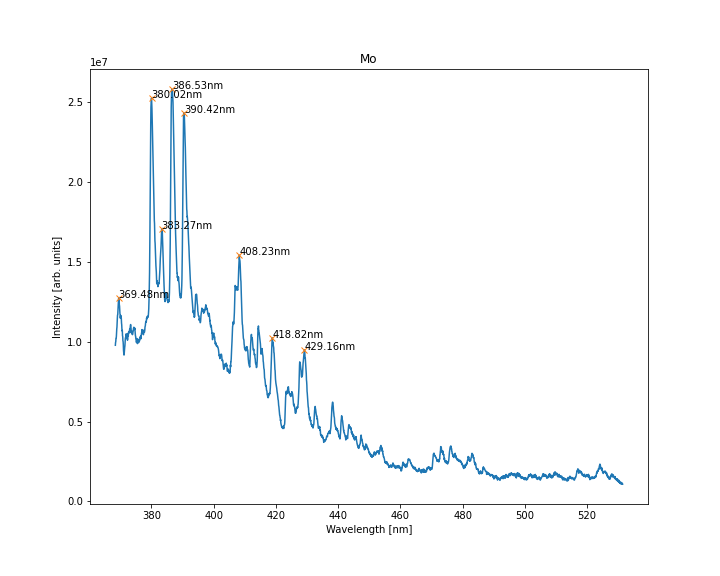
\includegraphics[scale=0.45]{Mo/Mo_450.png}
\end{frame}

\begin{frame}
    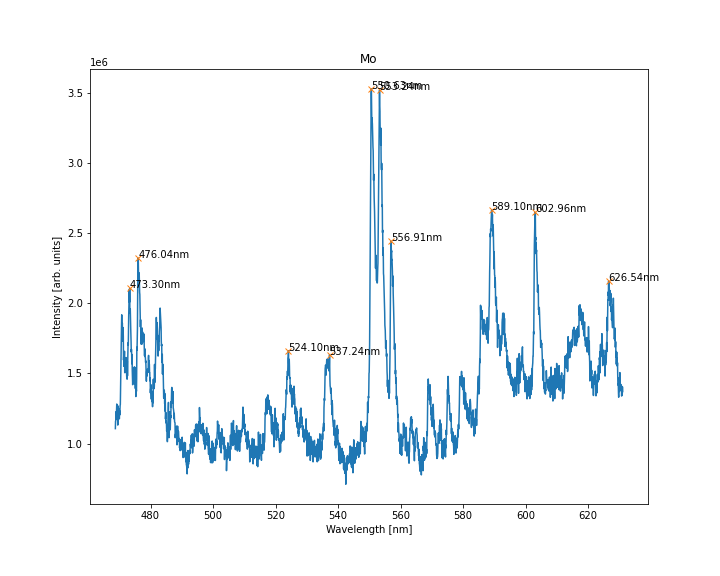
\includegraphics[scale=0.45]{Mo/Mo_550.png}
\end{frame}

\begin{frame}
    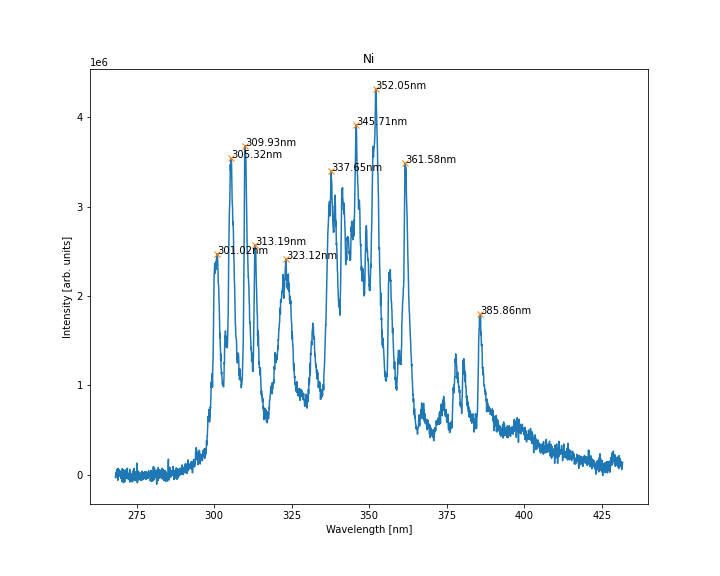
\includegraphics[scale=0.45]{Ni/Ni_350.png}
\end{frame}

\begin{frame}
    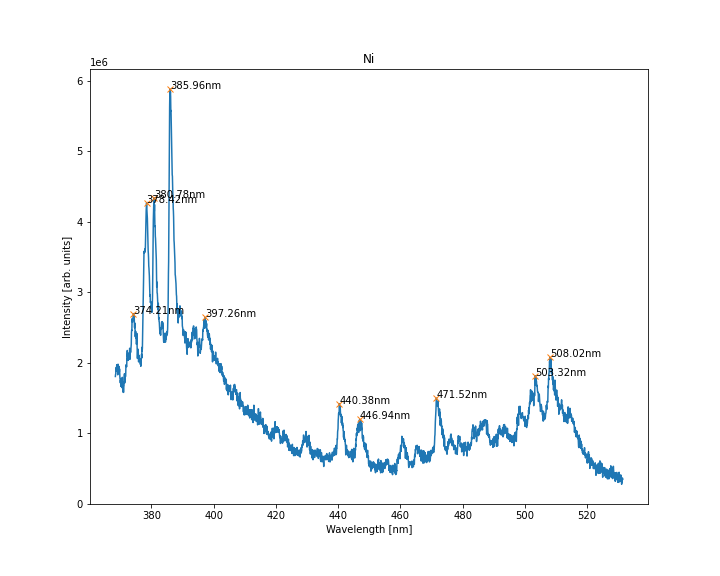
\includegraphics[scale=0.45]{Ni/Ni_450.png}
\end{frame}

\begin{frame}
    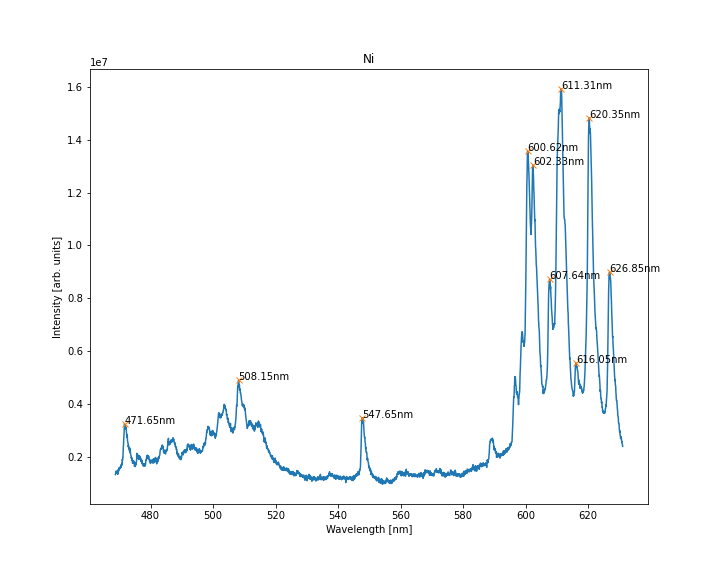
\includegraphics[scale=0.45]{Ni/Ni_550.png}
\end{frame}

\begin{frame}
    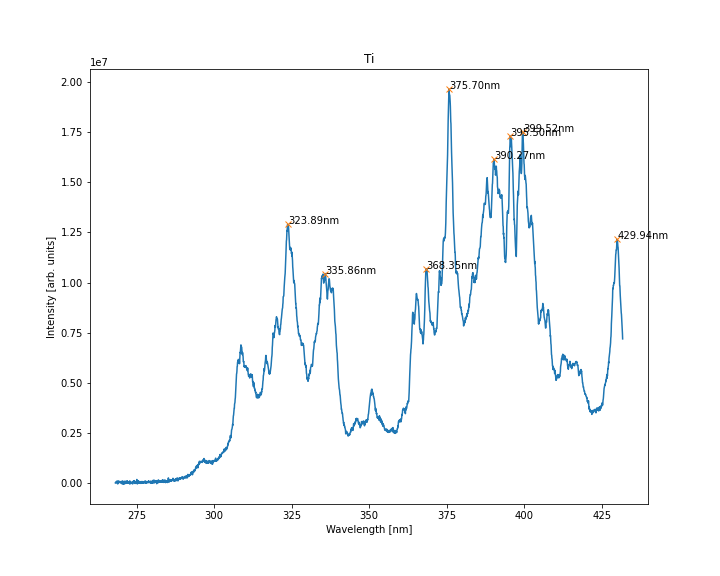
\includegraphics[scale=0.45]{Ti/Ti_350.png}
\end{frame}

\begin{frame}
    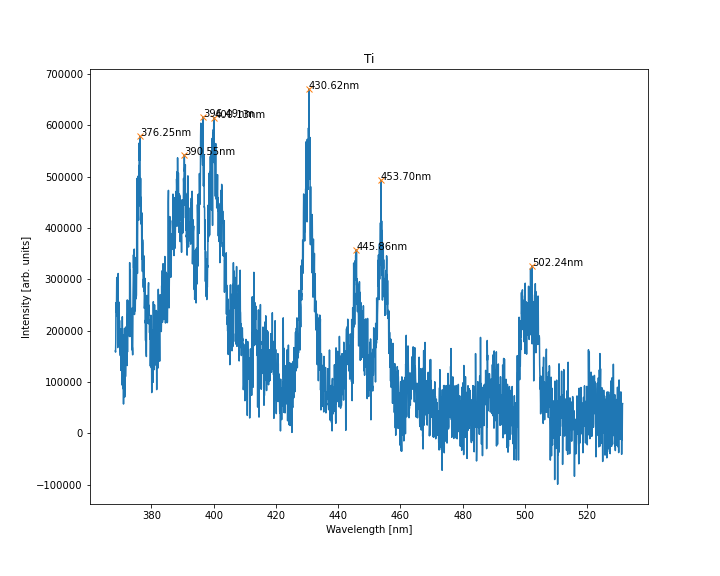
\includegraphics[scale=0.45]{Ti/Ti_450.png}
\end{frame}

\begin{frame}
    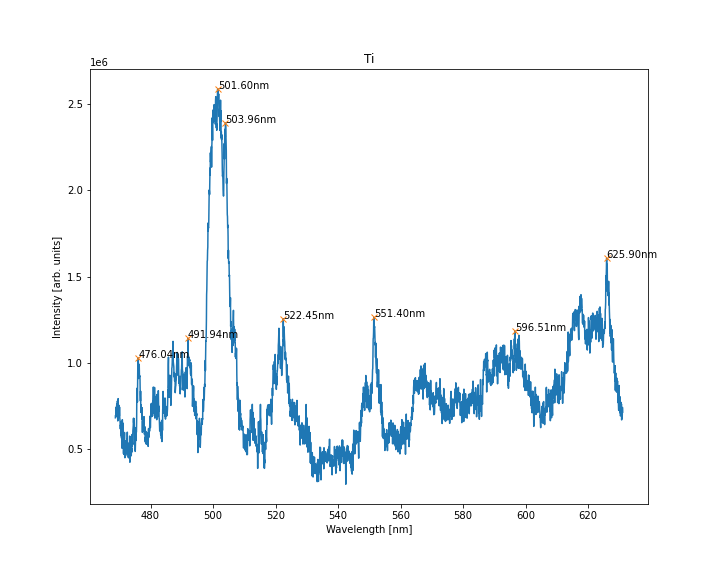
\includegraphics[scale=0.45]{Ti/Ti_550.png}
\end{frame}

\begin{frame}
    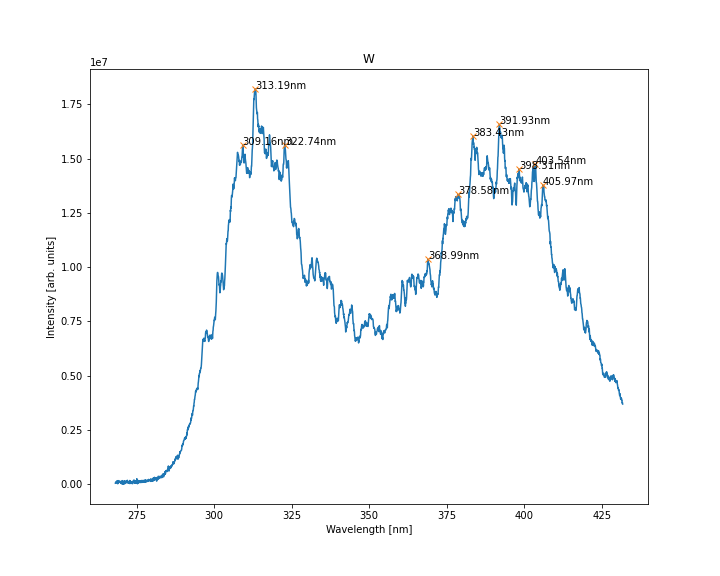
\includegraphics[scale=0.45]{W/W_350.png}
\end{frame}

\begin{frame}
    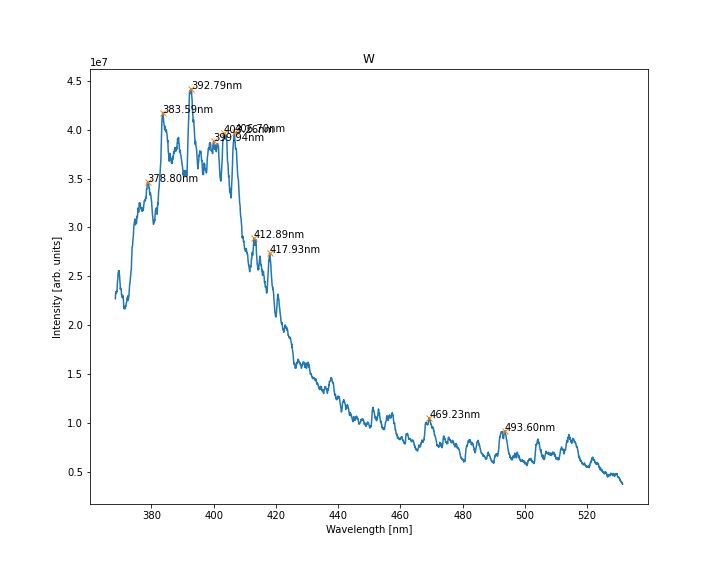
\includegraphics[scale=0.45]{W/W_450.png}
\end{frame}

\begin{frame}
    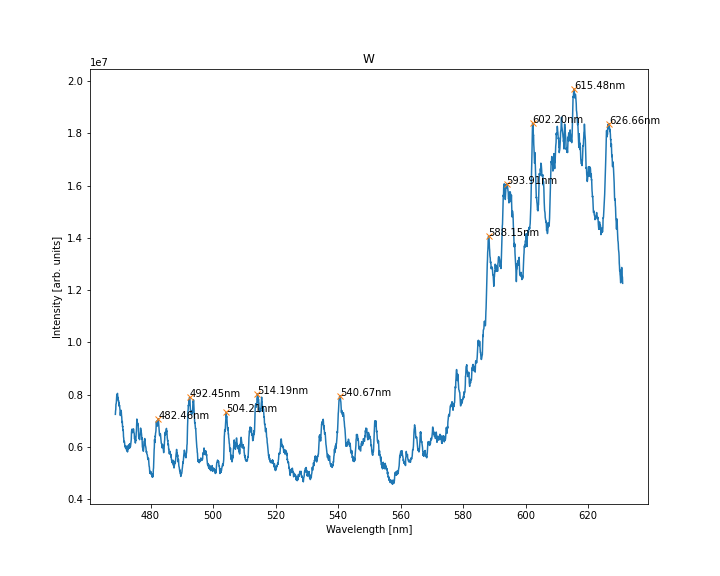
\includegraphics[scale=0.45]{W/W_550.png}
\end{frame}


\end{document}